\newpage
\section[Höhere Analysis]{Höhere Analysis}
\textit{Haben Teilmengen $A\subseteq \R^n$ eine kleinere Dimension $k<n$, dann verschwindet das Lebesgue-Maß. Allerdings kann man auch diesen Objekten sowas wie einen Flächeninhalt zuordnen. Voraussetzung dafür ist stets die Parametrisierbarkeit der Oberfläche, wir betrachten also Mannigfaltigkeiten. Der Trick it, dass man die Oberfläche $A$ durch eine Paramterisierung $\varphi: \R^k\rightarrow A$ auf eine Menge $\varphi^{-1}(A)$ zurückführt, deren Lebesgue-Maß nicht verschwindet.}
\subsection{Integration über Mannigfaltigkeiten}
\begin{Def}{Differenzierbare Kurven}
    Sei $\varphi: \R \rightarrow \R^2, t\mapsto \varphi(t)$ eine Kurve.
    \begin{center}
    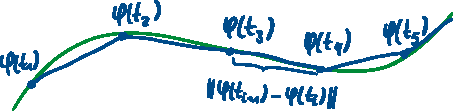
\includegraphics[width=0.65\textwidth]{Dateien/Linienintegral_1.pdf}
\end{center}
    Die Länge der Kurve zwischen zwei Werten $t_1<t_n$ kann approximiert werden durch
    $$v_1(\varphi)=\sum_{i=1}^{n-1}||\varphi(t_{i+1})-\varphi(t))||$$
    Schreibt man dies um, wählt gleich große Intervalle $\Delta t$ und bildet den Grenzwert $\Delta t \rightarrow 0$, erhällt man:
    $$v_1(\varphi)=\sum_{i=1}^{n-1}||\frac{\varphi(t_i+\Delta t)-\varphi(t_i)}{\Delta t}||\Delta t \rightarrow \int_{t_1}^{t_n}||\varphi'(t)||dt$$
    Dies lässt sich auf beliebige Dimensionen verallgemeinern. wir haben also schonmal eine Formel gefunden, mit der wir die Fläche von eindimensionalen Untermannigfaltigkeiten ausrechnen können:
    $$\int_M dS(x)=\int_{t_a}^{t_b}||\varphi'(t)||dt=\int_{t_a}^{t_b}\sqrt{\varphi_1(t)^2+\dots+\varphi_n(t)^2}dt$$
    Um also eine Funktion $f(x)$ entlang eines Weges $\varphi(t)$ zu integrieren, muss jedes Teilstück mit einem Funktionswert gewichtet werden:
    \begin{center}
    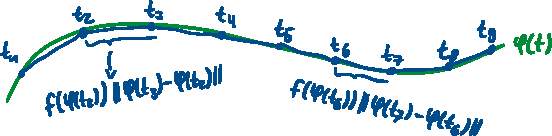
\includegraphics[width=0.65\textwidth]{Dateien/Linienintegral_2.pdf}
\end{center}
    Daraus folgt das \red{Linienintegral}:
    $$\int_M f(x) dS(x) \approx \sum_{i=1}^n f(\varphi(t_i))\frac{||\varphi(t_{i+1})-\varphi(t_i)||}{\Delta t}\Delta t= \int_{t_1}^{t_n}f(\varphi(t))||\varphi'(t)||dt$$
    Für allgemeine Mannigfaltigkeiten gilt die Formel:
    $$\int_M f(x)dS(x) = \int_T f(\varphi(t)) \sqrt{g(t)}d^kt$$
    wobei $$g(t)=\det((\braket{\partial_j \varphi(t), \partial_l \varphi(t)})_{1\leq j, l\leq k})$$ die \red{Gramsche Determinante} ist.
\end{Def}
Für eindimensionale Mannigfaltigkeiten gilt die nützliche Formel $g(t)=\braket{\partial \varphi(t), \partial \varphi(t)}=||\varphi ' (t)||^2$.
\begin{Def}{Gramsche Determinante}
    Die \red{Gramsche Determinante} ist die Determinante des Maßtensors
    $$g_{ij}(t)=\braket{\partial_i \varphi(t), \partial_j \varphi(t)} \quad (1\leq i,j\leq k)$$
    wobei $\varphi$ eine Karte (also eine homöomorphe Immersion) einer $k$-dimensionalen Untermannigfaltigkeit des $\R^n$ ist. 
\end{Def}
\begin{Beispiel}{Länge der Zykloide}
    Wir sollen die Länge $v_1(C)$ der Zykloide $C=\{ (t-\sin(t), 1-\cos(t)) | t\in [0,2\pi]\}$ berechnen. Die Zykloide ist die Bahn, die ein bestimmter Kreispunkt beim Abrollen des Einheitskreises auf der x-Achse beschreibt.
   \begin{center}
    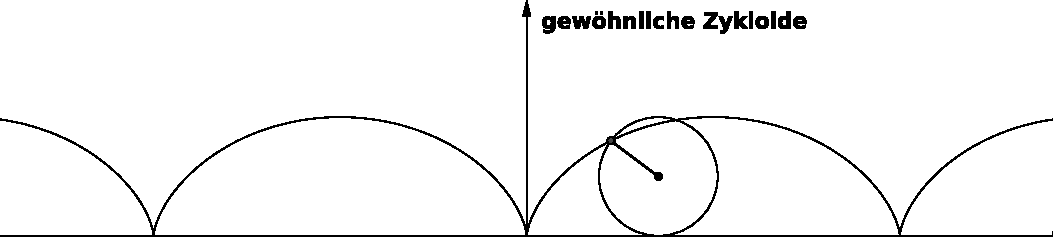
\includegraphics[width=0.8\textwidth]{Dateien/Zykloide.pdf}
\end{center}
$$\int_C 1 dS(x)=\int_{\text{Parametrisierung}} 1\cdot \varphi(t)\sqrt{g(t)}dt=\int_\varphi \sqrt{g(t)}dt$$
$$v_1(C)=\int_0^{2\pi} \sqrt{g(t)}dt$$
Für die Parametrisierung wählen wir einfach $\varphi(t)=(t-\sin(t),1-\cos(t))$. Dann müssen wir $g(t)=||\varphi'(t)||^2$ berechnen. 
$$\varphi'(t)=(1-\cos(t), \sin(t))$$
$$||\varphi'(t)||=\sqrt{\braket{\varphi ', \varphi '}}=\sqrt{(1-\cos(t))^2+\sin(t)}=\sqrt{1-2\cos(t)+\cos^2(t)+\sin^2(t)}$$
$$=\sqrt{2-2\cos(t)}$$
Nun können wir die Länge ausrechnen:
$$v_1(C)=\int_0^{2\pi} \sqrt{2(1-\cos(t))}dt=\int_0^{2\pi} \sqrt{1\sin^2(\frac{t}{2})}dt=4[\cos(\frac{t}{2})]^{2\pi}_0=8$$
\end{Beispiel}
\newpage
\subsection{Differentialformen}
Differentialformen bieten einen sehr abstrakten, aber auch sehr mächtigen Formalismus, um auf Mannigfaltigkeiten zu rechnen. Ich versuche hier die Idee anhand von Einsformen, auch Pfaffsche Formen genannt, klarzumachen, die für eindimensionale Mannigfaltigkeiten gelten und dann den Formalismus auf beliebige $k$-dimensionale Mannigfaltigkeiten zu erweitern.
\begin{Def}{Einsform}
    Die \red{Einsform} oder Pffafsche Form ist eine Funktion von einer offenen Menge $U\in \R^n$ nach $L(\R^n, \R)$. Sie ordnen jedem $x\in U$ eine lineare Abbildung zu. \\ \\
    Sei $n=1$, dann gilt:
    $$\omega_f: U\rightarrow L(\R, \R), \quad x\mapsto S_x(dx)=f'(x)\cdot dx$$
    Der Wert $x$ wird also auf eine Gerade mit der Steigung $f'(x)$ abgebildet, oder allgemein
    $$\omega= k\cdot dx$$
    Sei $n=2$
    $$\omega_f: U\rightarrow L(\R^2, \R), \quad x\mapsto \braket{\grad f(x), dx}$$
    Die allgemeine Einsform schreibt man also einfach als
    $$\omega = a_1\cdot dx_1+a_2\cdot dx_2$$

    Für $n=k$ erhalten wir also die Einsform $\omega = a_1 dx_1 + a_2 dx_2 + \dots + a_n dx_n$
\end{Def}
Das Integral einer Einsform $\omega=a\cdot dx$ auf dem Interval $I\subseteq \R$ ist definiert als $$\int_I \omega = \int_I a \cdot dx$$
\begin{Def}{$k$-Formen}
    Eine \red{$k$-Form} ist eine Differentialform der Gestalt:
$$\omega = a_1 \cdot dx_1\land dx_2 \land ... \land dx_k + c$$
wobei $c$ maximal eine $(k-1)$-Form ist und $\land$ das Dachprodukt.
\end{Def}

\begin{Def}{Integration über Mannigfaltigkeiten mit Differentialformen}
    Sei $M$ eine $k$-dimensionale Untermannigfaltigkeit in $U\subseteq \R^n$ und $\omega$ eine $k$-Form auf $U$. Sei $\varphi$ eine Karte von $M$. Dann gilt:
    $$\int_M \omega = \int_{\varphi^{-1}(M)}\varphi^*\omega$$
    $\varphi^*\omega$ ist der sogenannte Pullback oder auch Rücktransport. Er lautet:
    $$\omega = \sum_{1\leq j_1 <\dots < j_k\leq n} f_{j_1...j_k}dx_{j_1}\land ...\land dx_{j_k}$$
    $$\Rightarrow \varphi^* \omega = \sum_{1\leq j_1 < ... < j_k\leq n}(f_{j_1...j_k}\circ \varphi)d\varphi_{j_1}\land ...\land d\varphi_{j_k}$$
\end{Def}
\begin{Def}{Vektorielle Flächenelement}
        Das \red{vektorielle Flächenelement} wird definiert durch:
    $$d\vec{S}=(dS_1, ..., dS_n)^T$$
    $$\Rightarrow dS_i=(-1)^{i-1}dx_1\land ... \land \underset{\text{diese Komponente wird ausgelassen}}{\hat{dx_i}}\land ...\land dx_n$$
\end{Def}
\begin{Satz}{Satz}{Integration über Hyperflächen}

    Sei $M$ eine Hyperfläche im $\R^n$ mit dem Einheits-Normalen-Feld $\nu: M\rightarrow \R^n$. Sei $f=(f_1, ..., f_n)$ ein stetiges Vektorfeld. Für eine kompakte Teilmenge $K\subseteq M$ gilt:
    $$\int_K \braket{f, d\vec{s}}=\int_K \braket{f(x), \nu(x)}dS(x)$$
\end{Satz}
\begin{Def}{Ableitung von Differentialformen}
    Sei $\omega$ eine $k$-Form auf $U\subseteq \R^n$. Sind die Koeffizientenfunktionen $f_{j_1...j_k}$ differenzierbar, dann definiert man die Ableitung eine Differentialform durch:
    $$\omega = \sum_{1\leq j_1<...<j_k\leq n} f_{j_1...j_k}dx_{j_1}\land ... \land dx_{j_k}$$
    $$d\omega = \sum_{1\leq j_1<...<j_k\leq n} \sum^n_{j=1}\frac{\partial f_{j_1...j_k}}{\partial x_j}dx_j \land dx_{j_1}\land ...\land dx_{j_k}$$
\end{Def}
\begin{Def}{Geschlossen- und Exaktheit}
    $$d\omega = 0 \quad \Rightarrow \omega \text{ ist geschlossen}$$
    $$\exists \eta: d\eta = \omega \quad \Rightarrow \omega \text{ ist exakt}$$
    Außerdem ist jede auf $U\subseteq \R^n$ stetig differenzierbare exakte $k$-Form geschlossen.
\end{Def}
\begin{Satz}{Lemma}{Lemma von Poincaré}
    Jede auf einer \red{sternförmigen} (d.h. es gibt ein Punkt $x_0\in U$, sodass für jeden Punkt $x\in U$, die Verbindungsstrecke $\overline{xx_0}\in U$) offenen Teilmenge $U\subseteq \R^n$ geschlossene $k$-Form ist exakt.
\end{Satz}
\begin{Def}{Alternierende $k$-Form}
    Eine alternierende $k$-Form auf einem $\mathbb{K}$-Vektorraum $V$ ist eine multilineare Abbildung:
    $$\omega: V^k \rightarrow \mathbb{K}$$
    die verschwindet, sobald wenigstens zwei Argumente gleich sind:
    $$\exists i\neq j: v_i = v_j \Rightarrow   v_1\land v_2\land ... \land v_i \land ... \land v_j=0$$
    Der Raum aller $k$-Formen nennt man $1^kV^*$. Man setzt:
    $$\Lambda^0V^*=\mathbb{K} \quad \Lambda^1V^*=V^*$$
    Es gilt:
    \begin{itemize}
        \item $v_1\land v_2 = -v_2\land v_1$
        \item $\dim \Lambda^k V^* = \begin{pmatrix}
            \dim(V) \\ k
        \end{pmatrix}$
    \end{itemize}
\end{Def}
\begin{Beispiel}{Lineare Unabhängigkeit von Differentialformen}
Gegeben ist der Vektorraum $V$ mit der kanonischen 4D-Basis. Sind die Vektoren
$$x_1=v_1\land v_2\land v_4+ v_2\land v_1\land v_3$$
$$x_2=v_2\land v_4\land v_3 - v_1\land v_4\land v_3$$
$$x_3=v_2\land v_1 \land v_4$$
linear unabhängig? \\ \\
Dies können wir so überprüfen, indem wir die Indizes der Größe nach ordnen.
$$x_1=v_1\land v_2\land v_4- v_1\land v_2\land v_3$$
    $$x_2=v_1\land v_3\land v_4-v_2\land v_3\land v_4$$
$$x_3=-v_1\land v_2 \land v_4$$
Wir merken schon sofort, dass $\lambda_1 x_1+\lambda_2 x_2+\lambda_3 x_3=0$ nur wenn $\lambda_1, \lambda_2, \lambda_3 = 0$, also sind die Vektoren linear unabhängig.
\end{Beispiel}
\begin{Beispiel}{Rechnung mit dem Dachprodukt}
    Sei $V$ der Vektorraum mit einer Basis $\{v_1, v_2, v_3, v_4\}$ und sei $\{\varphi_1, \varphi_2, \varphi_3, \varphi_4\}$ des $V^*$ gegeben. Berechne 
    $((\varphi_1-\varphi_3)\land(\varphi_2+\varphi_4))(v_1-v_3, v_2+v_4)$.
    $$=\det\begin{pmatrix}
        (\varphi_1-\varphi_3)(v_1-v_3) & (\varphi_1-\varphi_3)(v_2+v_4) \\
        ((\varphi_2-\varphi_4)(v_1-v_3) & (\varphi_2-\varphi_4)(v_2+v_4))
    \end{pmatrix}$$
    $$=\det\begin{pmatrix}
        \varphi_1(v_1)-\varphi_3(v_1)-\varphi_1(v_3)+\varphi_3(v_3) & \varphi_1(v_2)-\varphi_3(v_2)-\varphi_3(v_4)+\varphi_1(v_4) \\
        \varphi_2(v_1)-\varphi_2(v_3)+\varphi_4(v_1)-\varphi_4(v_3) & \varphi_2(v_2)+\varphi_4(v_2)+\varphi_2(v_4)+\varphi_4(v_4)
    \end{pmatrix}$$
    $$=\det\begin{pmatrix}
        2 & 0 \\
        0 & 2
    \end{pmatrix}=4$$
\end{Beispiel}
\newpage 
\begin{Beispiel}{Präsenzaufgabe 3 aus dem Blatt 9}
    %Sei $U\subseteq \R^3$ offen. Seien außerdem $f,g: U\rightarrow \R$ beliebig oft differenzierbare Funktionen und $a,b: %U\rightarrow \R^3$ beliebig oft differenzierbare Vektorfelder. Betrachten Sie dann die folgenden Differentialformen: \\
    $\text{0-Form} \quad f,$ \\
    $\text{1-Form} \quad \eta=a_1 dx_1+a_2dx_2+a_3dx_3,$ \\
    $\text{2-Form} \quad \varphi=b_1dx_2\land dx_3 + b_2dx_3\land dx_1+b_3dx_1\land dx_2,$ \\
    $\text{3-Form} \quad \omega=gdx_1\land dx_2\land dx_3$ \\
    Wir sollen nun jeweils die äußere Ableitung berechnen und die Operatoren $\grad$, $\rot$, div unter Verwendung des %Volumenelements un der vektoriellen Linien-/Flächenelemente auswerten.
    $0$-Form:\\
    $$df=\frac{\partial f}{\partial x_1}dx_1+\frac{\partial f}{\partial x_2}dx_2+\frac{\partial f}{\partial x_3}dx_3$$
    Der Ausdruck $df$ erinnert sehr an die \red{Divergenz}.
    $$d\eta = da_1\land dx_1+da_2\land dx_2 + da_3\land dx_3$$
    $$={\frac{\partial a_1}{\partial x_1}dx_1\land dx_1} + \frac{\partial a_1}{\partial x_2}dx_2\land dx_1 + \frac{\partial a_1}{\partial x_3}dx_3\land dx_1) +$$ $$( \frac{\partial a_1}{\partial x_1}dx_1\land dx_2 + {\frac{\partial a_1}{\partial x_2}dx_2\land dx_2} + \frac{\partial a_1}{\partial x_3}dx_3\land dx_2) +$$ $$( \frac{\partial a_1}{\partial x_1}dx_1\land dx_3 + \frac{\partial a_1}{\partial x_2}dx_2\land dx_3 + {\frac{\partial a_1}{\partial x_3}dx_3\land dx_3)} $$
\begin{center}
        Alle Terme mit zwei gleichen Ableitungen sind gleich 0.
\end{center}

    $$d\eta = (\frac{\partial a_3}{\partial x_2}-\frac{\partial a_2}{\partial x_3})dx_2\land dx_3+(\frac{\partial a_1}{\partial x_3}-\frac{\partial a_3}{\partial x_1})dx_3\land dx_1+(\frac{\partial a_2}{\partial x_1}-\frac{\partial a_1}{\partial x_2})dx_1\land dx_2$$
    Der Ausdruck $d\eta$ erinnert sehr an die \red{Rotation}.
    $$d\varphi=(\frac{\partial b_1}{\partial x_1}+\frac{\partial b_2}{\partial x_2}+\frac{\partial b_3}{\partial x_3})dx_1\land dx_2 \land dx_3$$
    Und $d\varphi$ an den \red{Gradienten}.
    $$\omega = dg\land dx_1\land dx_2\land dx_3 = 0$$
\end{Beispiel}
\begin{Def}{Glatter Rand}
    Ist $A\subseteq \R^n$ kompakt, dann sagen wir, dass $A$ einen glatten Rand hat, wenn $\forall a\in \partial A$  eine offene Umgebung $U\subseteq \R^n$ existiert und eine stetig differenzierbare Funktion $\Psi: U\rightarrow \R$, sodass 
    \begin{itemize}
        \item $A\cap U = \{x\in U | \Psi(x)\leq 0\}$
        \item $\grad \Psi(x) \neq 0 \quad \forall x \in U$
    \end{itemize}
       \begin{center}
    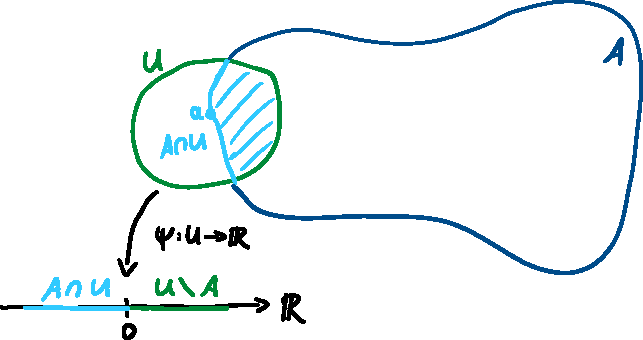
\includegraphics[width=0.6\textwidth]{Dateien/Glatter_Rand.pdf}
\end{center}
\end{Def}
\begin{Beispiel}{Kugel}
    Wir betrachten die Menge $\overline{B_R(0)}=\{(x,y,z)\in\R^3, x^2+y^2+z^2\leq R\}$. Außerdem betrachten wir die Funktion $\Psi: \R^3\rightarrow \R, (x,y,z)\mapsto x^2+y^2-z^2-R$. \\ \\
    Sie ist stetig diff'bar und es gilt $$\R^3\cap \overline{B_R(0)}=\{\Psi(x,y,z)\leq 0\}$$
    Außerdem finden wir immer Umgebungen $U$ von Randpunkten, sodass $(0,0,0)\notin U$ und daher gilt:
    $$\grad \Psi=2\begin{pmatrix}
        x \\ y \\ z
    \end{pmatrix}\neq 0$$
    Also hat $\overline{B_R(0)}$ einen glatten Rand.
\end{Beispiel}
\begin{Def}{Einheits-Normalenfeld}
    Wir betrachten ein Kompaktum $A$ mit glattem Rand $\partial A$. Dann gilt für $\forall a \in \partial A, \exists\nu(a)\in \R^n:$
    \begin{enumerate}
        \item $\nu(a)$ steht senkrecht auf dem Tangientialraum $T_a(\partial A)$ der $(n-1)$-dimensionalen Untermannigfaltigkeit $\partial A$.
        \item Der Vektor $\nu(a)$ ist ein Einheitsvektor $||\nu(a)||=1$.
        \item $\exists \epsilon >0: a+t\nu(a)\notin A \quad \forall t\in (0,\epsilon)$.
    \end{enumerate}
\end{Def}
\newpage
\subsection{Wichtige Integralsätze der Vektoranalysis}
Das meiste hier sollte euch schon aus der Physik 2 bekannt sein. Wir starten mit der Wiederholung von drei wichtigen Begriffen.
\begin{Def}
{Rotation}
Mithilfe des Vektorproduktes können wir nun durch $\rot:\mathbb{R}^3\to\mathbb{R}^3$ eine weitere Abbildung für Vektorfelder $\Fvec:\mathbb{R}^3\to\mathbb{R}^3$ definieren:
\begin{equation}
    \rot \Fvec:=\Matrix{\partial_2 F_3-\partial_3 F_2\\\partial_3 F_1-\partial_1 F_3\\\partial_1 F_2-\partial_2 F_1}=\nablavec\times \Fvec,
\end{equation}
wobei wir $\nablavec:=\MatrixInline{\partial_1\\\partial_2\\\partial_3}$ als Abkürzung gewählt haben.
\end{Def}
\begin{Beispiel}
{Rotation}
Für die oben schon betrachtete, auf $\mathbb{R}^3$ erweiterte Abbildung $\Fvec:\mathbb{R}^3\to\mathbb{R}^3,\,\Fvec(x,y,z)=\MatrixInline{-y\\x\\0}$ ergibt sich $\rot \Fvec=\MatrixInline{\partial_y 0-\partial_zx\\\partial_z (-y)-\partial_x 0\\\partial_x x-\partial_y (-y)}=\MatrixInline{0\\0\\2}$.\\
Unabhängig davon, wo wir uns befinden, rotiert das Feld um die $z$-Achse entgegen\footnote{also mathematisch positiv} des Uhrzeigersinnes.
\end{Beispiel}
\begin{Def}
{Divergenz}
Wir nennen ein Vektorfeld $F:\mathbb{R}^n\to\mathbb{R}^n$ partiell differenzierbar, wenn jede Komponentenfunktion partiell differenzierbar ist.\\
Die Abbildung $\divv:\mathbb{R}^n\to\mathbb{R},\,F(\xvec)\to\divv(F(\xvec))=\sum_{i=1}^n\partial_iF_i(\xvec)$ nennen wir \red{Divergenz} von $F$.
\end{Def}
\begin{Beispiel}
{Anschauung zur Divergenz}
\begin{itemize}
    \item Betrachte $F:\mathbb{R}^2\to\mathbb{R}^2,\,F(x,y)=\MatrixInline{-y\\x}$, so ist $\divv F=\partial_x(-y)+\partial_y(x)=0$.
    \item Betrachte $F:\mathbb{R}^2\to\mathbb{R}^2,\,F(x,y)=\MatrixInline{x\\y}$, so ist $\divv F=2$.
\end{itemize}
\blue{Die Divergenz im Punkt $\xvec$ sagt uns, wie stark die Vektoren des Vektorfelds dort \textit{auseinanderdriften}.}
\end{Beispiel}
\begin{Def}
{Gradient}
Den $n\times 1$-Vektor $\grad f=\MatrixInline{\partial_{x_1}f\\\vdots\\\partial_{x_n}f}$, der zeilenweise die partiellen Ableitungen von $f$ enthält, nennen wir \red{Gradienten} von $f$.
\end{Def}
\begin{Beispiel}
{Gradient einer Funktion}
Für die obige Funktion $g=xy^2\cos(x)$ ist
\begin{equation*}
    \grad f=\Matrix{\partial_x f\\\partial_y f}=\Matrix{y^2\cos(x)-xy^2\sin(x)\\2xy\cos(x)}.
\end{equation*}
\end{Beispiel}

Jetzt geht es mit der Vektoranalysis weiter.

\begin{Satz}{Satz}{Satz von Gauß}
    Sei $A$ ein Kompaktum mit stückweise glattem Rand $\partial A$, $\nu: \partial A\rightarrow \R^n$ das äußere Einheits-Normalenfeld und $F:U\rightarrow \R^n$ ein stetig diff'bares Vektorfeld, so gilt:
    $$\int_A \divv F(x)d^nx=\int_{\partial A}\braket{F(x), \nu(x)}dS(x)$$
    Alternativ sei $\omega=\braket{F, d\vec{s}}$, dann gilt:
    $$d\omega=(\divv F)\cdot dx_1\land ...\land dx_n$$
    $$\int_A \divv F d^nx=\int_A d\omega=\int_{\partial_M A}\braket{F, d\vec{s}}=\int_{\partial A}\braket{F,\nu}dS(x)$$
\end{Satz}
\begin{Satz}{Satz}{Satz von Stokes}
    Sei $M\subseteq U$ eine zweidimensionale Untermannigfaltigkeit durch ein Einheitsnormalenfeld $\nu: M\rightarrow \R^3$ orientiert ist. $A\subseteq M$ ist kompakt mit glattem Rand $\partial A$ und $F:U\rightarrow \R^3$ ein stetig diff'bares Vektorfeld. Dann gilt:
    $$\int_{\partial A}\braket{F, d\vec{s}}=\int_A\braket{\rot F(x), \nu(x)}dS(x)$$
    Alternativ sei $d\omega=\braket{\rot F, d\vec{s}}$ und $\varphi: [a,b]\rightarrow M$ ein positiv umlaufte Randweg (eine Parametrisierung), dann gilt:
    $$\int_A\braket{\rot F(x), d\vec{s}}=\int_A d\omega =\int_{\partial_M A} \omega =\int_{[a,b]}\braket{F(\varphi(t), \varphi'(t)}dt$$
\end{Satz}
\begin{Beispiel}{Anwendung des Satzes von Gauß}
    Berechne $\int\int_{\partial A} F\cdot d\vec{S}$ von $F=(3x+z^{77}, y^2-\sin(x^2z), xz+ye^{x^5})$, wobei $\partial A$ die Oberfläche eines Würfels mit den Dimensionen $0\leq x \leq 1$, $0\leq y\leq 3$ und $0\leq z\leq 2$ ist. \\ \\
    Die Berechnung dieses Integrals wäre sehr mühesam, aber zum Glück ist $$\divv F = 3+2y+x$$ Wenden wir nun den Satz von Gauß an:
    $$\int_{\partial A}  F d\vec{S} =\int\int\int_A \divv F dV$$
    $$=\int_0^1 dx \int_0^3 dy \int_0^2(3+2y+x)dz=39$$
\end{Beispiel}
\begin{Beispiel}{Anwendung des Satzes von Stokes}
    Benuzte den Satz von Stokes um $\int\int_S \rot F \cdot d\vec{S}$ von $F=y\vec{i}-x\vec{j}+yx^3\vec{k}$ zu berechnen, wobei $S$ die Spähre mit Radius 4 im Ursprung mit $z\geq 0$ ist.
          \begin{center}
    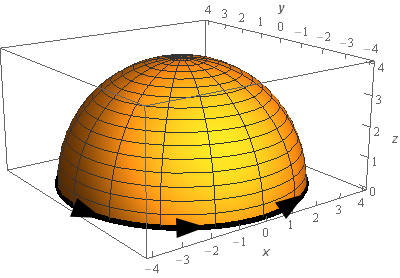
\includegraphics[width=0.5\textwidth]{Dateien/Stokes1.png}
\end{center}
Wir müssen nun eine parametrisierende Kurve finden. Es eignet sich der Weg am Rande der Kugel auf der Ebene $z=0.$
          \begin{center}
    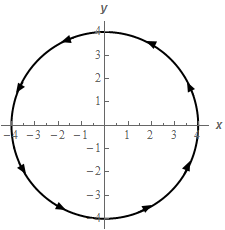
\includegraphics[width=0.3\textwidth]{Dateien/Stokes2.png}
    \end{center}
    $$\vec{r}(t)=(4\cos(t), 4\sin(t), 0) \quad 0\leq t \leq 2\pi$$
    Wir wenden nun den Satz von Stokes an.
    $$\int\int_S \rot F\cdot d\vec{S}=\int F(\vec{r}(t))\cdot\vec{r}(t)'dt $$
    $$F(\vec{r}(t))=(y, -x, yx^3)=(4\sin(t),-4\cos(t), 256\sin(t)\cos^3(t))$$
    $$\vec{r}(t)'=(-4\sin(t), 4\cos(t),0)$$
    $$F(\vec{r}(t))\cdot \vec{r}(t)'=-16\sin^2(t)-16\cos^2(t)=-16$$
    $$\int\int_S \rot F\cdot d\vec{S}=\int_0^{2\pi} -16dt = -32\pi$$
\end{Beispiel}
\begin{Beispiel}{Anwendung des Satzes von Green}
Der \red{Satz von Green} besagt:
$$\int_A(\frac{\partial}{\partial x_1}F_2(x)-\frac{\partial}{\partial x_2}F_1(x))dx_1dx_2=\int_{\mbox{Randweg $\alpha$}}\braket{F(s), d\vec{s}}, \mbox{ mit $d\vec{s}(t)=\alpha'(t)dt$}$$
Tatsächlich ist der Satz von Green eine 2D-Version des Satzes von Stokes, jedoch ist dieses Beispiel für die Klausur sehr nützlich. \\ \\
Wir sollen nun mit dem Satz und einem passend gewählten Vektorfeld ($F:\R^2\rightarrow \R^2$ den Flächeninhalt $I$ der von der Kurve $\alpha:[-1,1]\rightarrow\R^2$ umschlossenen Fläche, wobei $\alpha(t)=(t^2-1, t-t^3)$. Skizzieren sie dafür zunächst die Fläche.
\begin{center}
        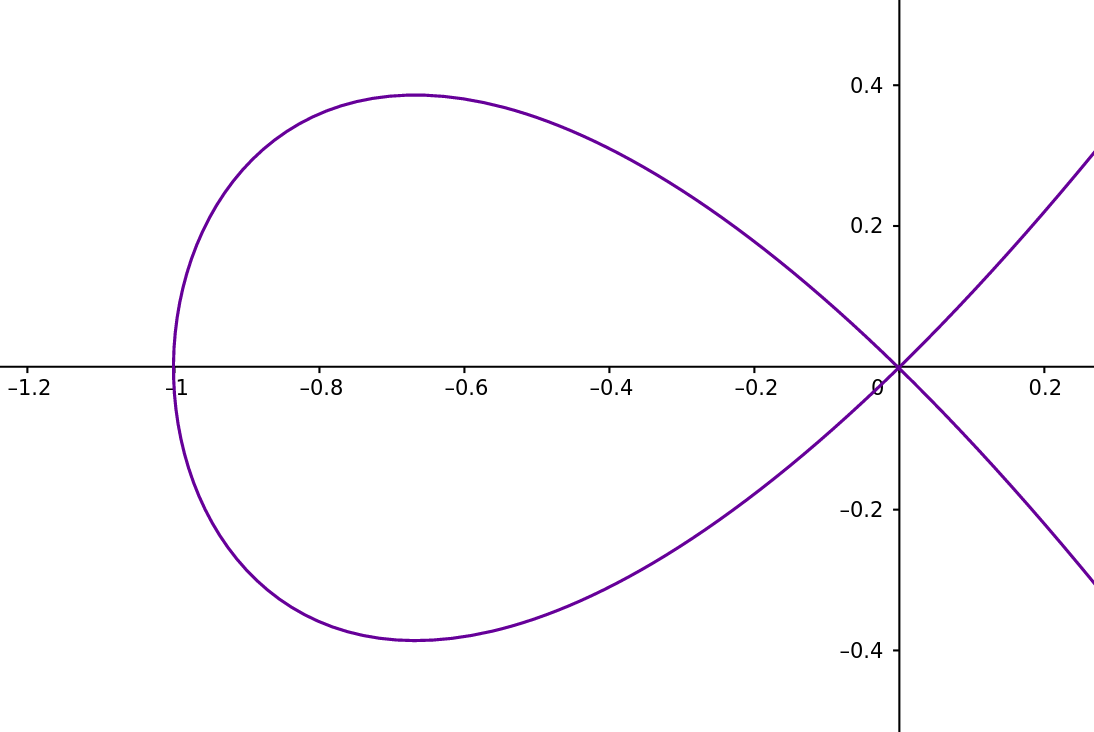
\includegraphics[width=0.65\textwidth]{Dateien/Green.png}
\end{center}
Wir müssen zuerst $\alpha'(t)$ und $F(\alpha(t))$ bestimmen.
$$\alpha'(t)=(2t,1-3t^2)$$
$$F(\alpha(t))=\begin{pmatrix}
    0 \\
    -\alpha_x
\end{pmatrix}=\begin{pmatrix}
    0 \\
    1-t^2
\end{pmatrix}$$
Nun berechnen wir $\braket{F(s), d\vec{s}}$
$$\braket{F(s), d\vec{s}}=\braket{F(\alpha(t)), \alpha'(t)dt}=\begin{pmatrix}
    0 \\
    1-t^2
\end{pmatrix}\cdot \begin{pmatrix}
    2t \\
    t-t^3
\end{pmatrix}dt=(1-t^2)(t-t^3)dt$$
Nun müssen wir nur noch integrieren:
$$I=\int_{-1}^{1} t^5-2t^3+t=\frac{8}{15}$$
\end{Beispiel}